% ====================
\chapter{Object Placement to Minimize Obstructions}
\label{ch:identify}
% ====================

% • In a paper you MUST provide the details, but FIRST convey the idea
% • Introduce the problem, and your idea, using EXAMPLES and only then
% present the general case
% • Explain it as if you were speaking to someone using a whiteboard
% • Conveying the intuition is primary, not secondary
% • Once your reader has the intuition, she can follow the details (but not vice
% versa)
% Even if she skips the details, she still takes away something valuable
% Evidence
% • Your introduction makes claims; The body of the paper provides evidence to
% support each claim
% • Check each claim in the introduction, identify the evidence, and forward-
% reference it from the claim
% • Evidence can be: analysis and comparison, theorems, measurements, case
% studies

\section{Design Goals}
We wish to identify a configuration of an object given an obstacle map.
Formally, (state spaces of each)

% ====================
\section{Preprocessing Finding Feasible Configurations}
\label{sec:feasibleparkingspot}
% ====================


From a ground map and object map, a set of feasible configurations for the
wheelchair are found. A wheel chair configuration is defined as $(x,y,\theta)$,
where $(x,y)$ define the centre of the wheelchair in the 2D map coordinates of
the ground and object map, and $\theta$ defines a rotation of the wheelchair,
where $\theta = 0$ is the angle of the wheelchair when the point cloud is
captured. Possible values of $\theta$ range from $-10$ to $10$ degrees (TODO
change).

To determine if each configuration is feasible, three checks are performed, as
seen in algorithm \autoref{alg:feasibilitycheck}. 

The first check is to see if the wheelchair
collides with any objects or is placed on areas not known to be ground. This
performed by checking if each configuration is fully within the ground map area.

The second check is to determine if each configuration can be reached from the
wheelchair's current configuration, the origin $(x_0,y_0,\theta_0)$. $(x_0,y_0)$
is determined from the same transformation used in
\autoref{sec:processingPointCloud} to align the ground plane to the x-y axes.
$\theta_0$ is set to $0$. 
This state is dilated to include a set of states within a 1 m radius: if any
state is connected to a state within 1 m of the wheelchair, it is deemed
feasible. This is done to accomodate for the minimum depth of the RGBD sensor.


A flood-fill algorithm is then performed on the
feasible configuration set obtained in the first check to determine all connect
feasible configurations to the origin $(x_0,y_0,\theta_0)$. Two feasible
configurations are deemed connnected if they are within one manhattan unit of
each other in $x-y-\theta$ space.
Then, feasible configurations from the first check that have no feasible
connecting path to the origin are deemed unreachable and discarded. 
This simplification assumes the possible transitions between states are a one
unit change in $x$, $y$ or $\theta$ (in effect, a holonomic system). 
Primitive transition curves of a differential drive system
\cite{balkcom2002time} has been developed, but this assumes no objects present.
The ease of computation justifies this choice.

Piano mover's problem/ holonomic system.


The third check ensures the entirety of the wheelchair falls within the bounds
of the map. TODO better description.

\begin{algorithm}
\caption{TODO Feasibility Check}
\label{alg:feasibilitycheck}
\begin{algorithmic}[1]
\Require{$groundMap, wheelChairMaps, origin$}
\Statex
\Function{FeasibleStates}{$groundMap, wheelChairMaps, origin$}
    \State $feasibleStates \gets$ 1 for all states
    \For{each configuration $c \in$ Configuration Space}
        \State $w \gets wheelChairMaps(c)$ TODO ?
        \State $feasibleStates(c) \gets$ 0 if $w$ is not enclosed in $groundMap$
        \State $feasibleStates(c) \gets$ 0 if $c$ is not connected in configuration space to $origin$
        \State $feasibleStates(c) \gets$ 0 if $w$ collides with edge of map
    \EndFor
\EndFunction
\Statex
\Ensure{$feasibleStates$, a 3D boolean array with values of $1$ representing
feasible configurations of the wheelchair}
\end{algorithmic}
\end{algorithm}

% ====================
\section{Choosing a Value Function to Maximizing Free Space Quality}
\label{sec:choosingparkingspot}
% ====================

So

Given the set of feasible parking spots, we must now choose one of them. What
defines a good parking spot? One could pose this as a supervised learning
problem, given many expert-labeled parking spots on different feasible
configuration sets \cite{wu2006parking, true2007vacant}. 
Obtaining meaningful labels when parking spots are not marked, however, is
challenging due to the shear number of possibilities of feasible configuration
sets. A reinforcement learning approach requires defining an appropriate reward
function, which brings us back to the problem of what defines a good parking
spot. We take a heuristics-based approach to develop a potential (reward)
function that is exhaustively evaluated for every configuration. This obtains a
full potential function for the state space, instead of a single state. The best
state may be chosen by taking the state with the maximum potential.

A good potential function will satisfy the following properties
\begin{itemize}
\item monotonically increasing, allowing for efficient computation
using gradients
\end{itemize}

TODO place in a general framework

We evaluate multiple approaches. We then determine performance based on an
empirical evaluation.

Algorithm \autoref{alg:generatestatepotentials} shows how a score is given to each
feasible configuration, where higher values correlate to more desirable parking
spots. $w$ in line 3 is a boolean 2D array with values of $1$ representing the
wheelchair at configuration $c$. A squared distance transform is then performed
on the union of $objectMap$ and $w$. This results in $distanceMap$ being the
squared distance of each ground pixel to the closest object to it (with the
wheelchair itself considered an object). This gives a score to each ground pixel:
the farther away the pixel is from all objects, the more desirable the ground
pixel. 

The squared term is included to quadratically favour ground pixels far
away from all objects. This can be reasoned that ground close to objects are less
desirable in a typical wheelchair environment: small areas and cracks between
obstacles are prohibitively small for humans or robots to pass through, and
ground directly next to obstacles risk collision. Ground far from obstacles, on
the other hand, allow for unobstructed movement and ample parking space for
other wheelchairs.

The score for each configuration is then the sum of all the scores for each
ground pixel, as in line 5.

\begin{algorithm}
\caption{Generating State Potentials}
\label{alg:generatestatepotentials}
\begin{algorithmic}[1]
\Require{$groundMap$, $objectMap$}
\Statex
\Function{GenerateStatePotentials}{$objectMap, wheelChairMaps, feasibleStates$}
    \For{each configuration $c \in feasibleStates$}
        \State $w \gets wheelChairMaps(c)$
        \State $distanceMap \gets$ squared distance transform of $objectMap \cup w$
        \State $statePotentials(c) \gets$ sum over all values of $distanceMap$
    \EndFor
\EndFunction
\Statex
\Ensure{$statePotentials$, a configuration-space array where each value
represents the desirability of that configuration.}
\end{algorithmic}
\end{algorithm}

\autoref{fig:desirabilityfunction} shows an example of state potentials
generated from Algorithm \autoref{alg:generatestatepotentials}.

\begin{figure}
\centering
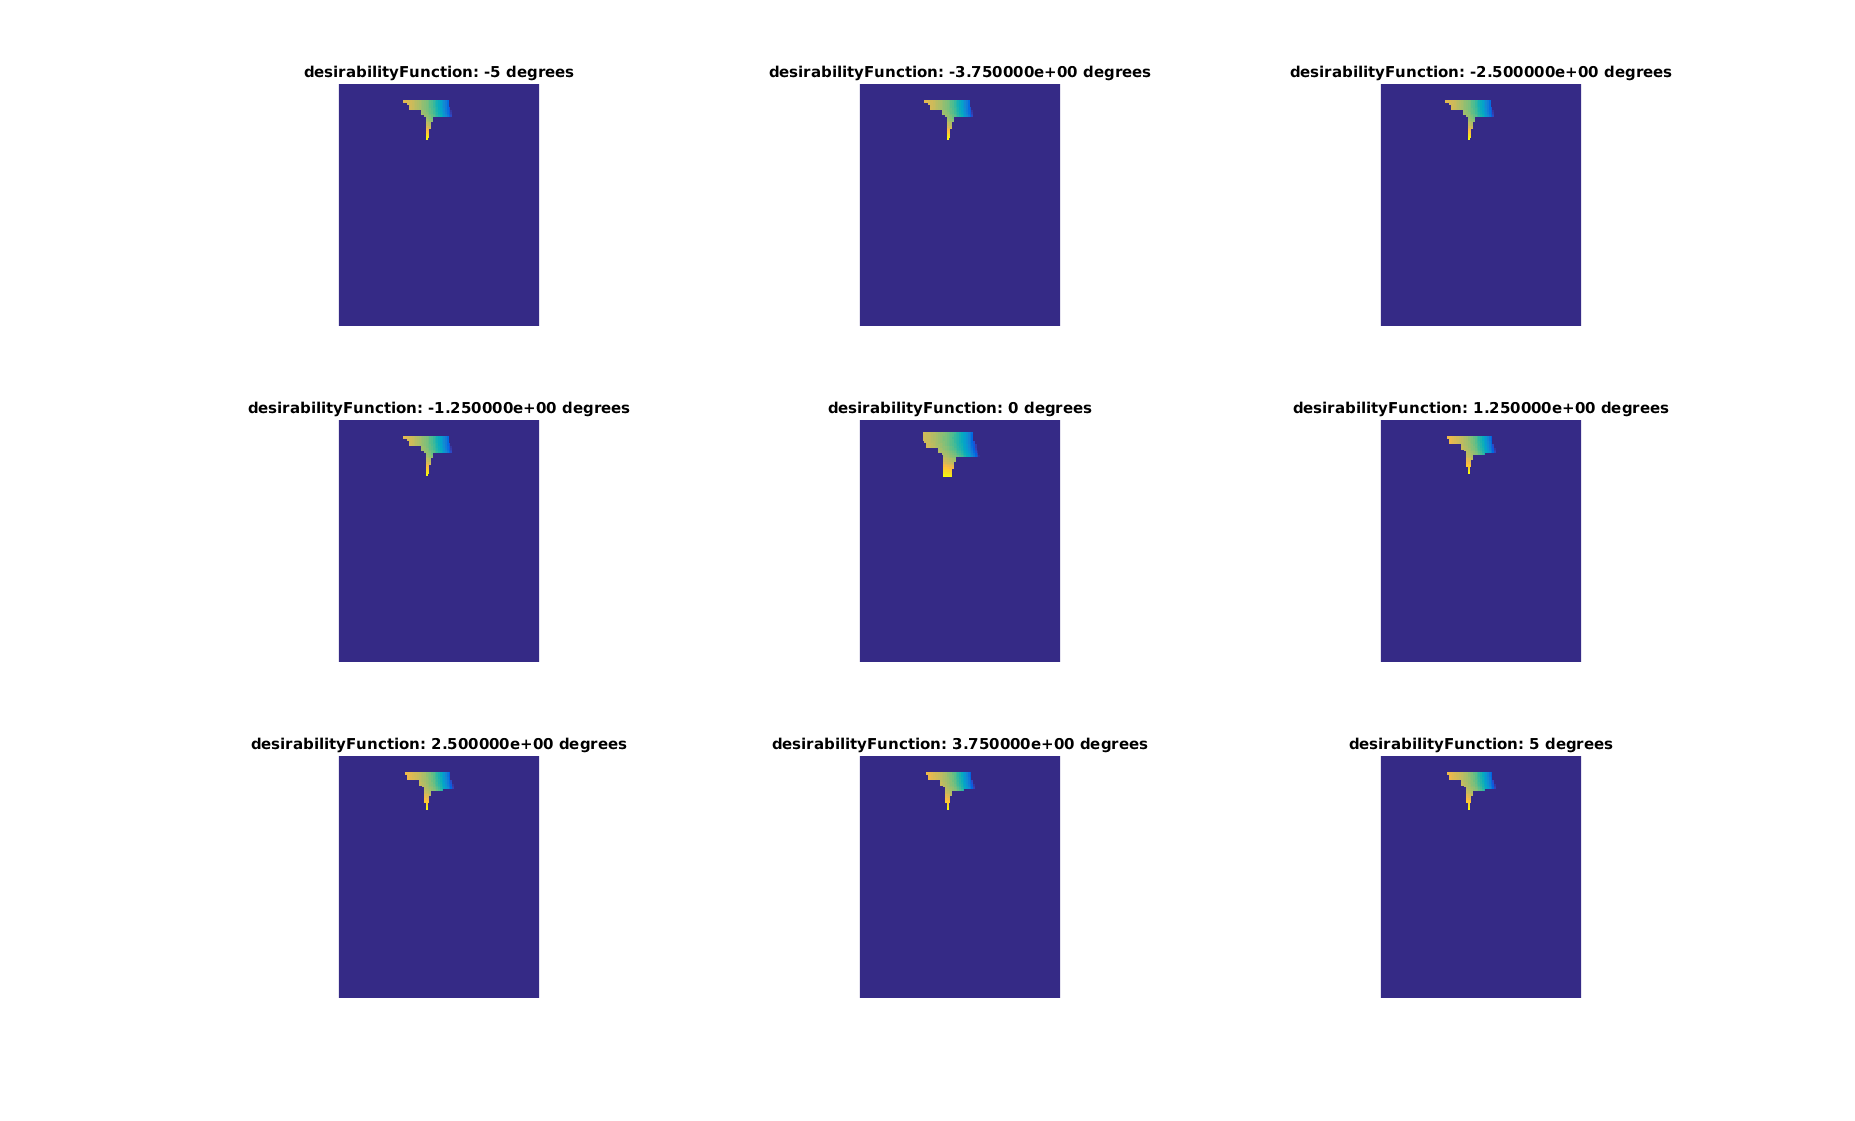
\includegraphics[width=6in]{figures/desirabilityfunction.png}
\caption{Example of a desirability function over a configuration space with 9
different values for $\theta$. Blue (dark) represents low desirability, yellow
(light) represents high desirability. Infeasible configurations determined in 
\autoref{sec:feasibleparkingspot} have desirabilities of $-\infty$.} 
\label{fig:desirabilityfunction}
\end{figure}

% ====================
\section{Efficent Value Function Calculation}
% ====================
% --------------------
\subsection{Distance Transforms}
% --------------------
From \cite{felzenszwalb2004distance}:
A distance transform of a binary image specifies the distance from each pixel to
the nearest ``on" pixel. Distance transforms are an important tool in computer
vision, image processing and pattern recognition.
Let $P$ be a binary image. Then for each pixel $p$, the distance transform is
defined as:

$$\mathcal{D}_{g(x)}(p) = \min_{q \in g(x)} d(p,q) $$

% --------------------
\subsection{Sliding Window Distance Transforms}
% --------------------
We introduce a linear-time algorithm for solving a class of problems that involve
calculating distance transforms with a sliding window. These problems can be
viewed as constrained case of ($+$,$\min$)-convolutions of two distance
transform functions. 
$Y$ is the space of pixels.
$P$ is a subset of $Y$ that is on.

Let us define ($+$,$\min$)-convolutions as: (todo fix)

$$ (f \oplus g) (x) = \sum_{x = -\infty}^\infty \min_{q \in [g(x) \cup f(x - p)]} d(p,q) $$


We implement min-convolutions in an efficient way.
Calculate the wheelchair distance transform for each configuration that's 2x as big in each dimension.
Calculate the obstacle map distance transform.
On a GPU for each configuration, select a subset of the distance transform that
matches the (x,y) location, and element-wise min with the obstacle map DT, then
take the sum. Selecting is constant time, $n$ mins is $n$ time, and sum is $n$
time, making it run in $2n = O(n)$ time, where $n$ is the number of pixels. This
is also easily parallelizable for each pixel, allowing for real-time operation.

Like the FFT for ($+$,$\times$)-convolution (normal convolutions) and generalized distance
transforms for constrained ($\min$,$+$)-convolutions, we introduce an efficient
algorithm to calculate ($+$,$\min$)-convolutions of distance transforms,
taking advantage of the following property of distance transforms:

$$DT(X \cup Y) = \min(DT(X), DT(Y))$$

Where $X$ and $Y$ are $n \times m$ binary images.
We note that $DT(Y)$ is constant for all configurations, and can be stored in
memory. $DT(X)$ varies for values of $X$, but we note that we can store a larger
array of $X$ which stores the value of every configuration of $X$.

% --------------------
\subsubsection{Min Convolutions}
% --------------------
From \cite{burcsi2010table}:
Let $x = (x_0, x_1, ..., x_n)$ and $y = (y_0, y_1, ..., y_n)$ be one-dimensional
vectors.
A min-convolution (also known as the (min,+)-convolution) of $x$ and $y$ is the
vector $x \star y = z = (z_0, z_1, ...,z_{2n})$
with $z_m = min(x_i + y_{m-i})$, where the minimum is taken over all possible
values of $i$. 
In contrast, standard convolution, or (+,*)-convolution, is obtained if min is replaced by $\sum$ and
$x_i + y_{m-i}$ by $x_i * y_{m-i}$ , i.e. 
$z_m = \sum(x_i * y_{m-i})$

What I want is (+,min)-convolution, $z_m = \sum min(x_i , y_{m-i})$

I can do this by:
making function A positive, function B negative.
Apply min-convolution.
making function A negative, function B positive.
Apply min-convolution.
do something else.


The only special case we are aware of where a fast algorithm is known for
rank-convolutions is the case when the mask is an axis-parallel box. This case
is common in computer vision and image processing. Rank-convolutions in this
case can be computed in O ( n log n) time; and min- convolution in O ( n) (Gil
and Werman [15]) \cite{babai2009computing}.

Computing min-convolutions when f is arbitrary but g is convex has received
special attention because of its applications to sequence alignment [9] and to
computing distance transforms of images [10]. As pointed out by Eppstein [9],
the problem can be solved in O ( n) time by using the totally monotone matrix
search algorithm of Aggarwal et al. [1].
\cite{babai2009computing}

Felzenszwalb and Huttenlocher [10] developed a different algorithm for the case
when g is convex by noting the relationship between min-convolutions and
lower-envelopes (minimum of a family of functions). The same approach can be
used when g is concave. This algorithm runs in O ( n) time if an intersection
point between shifted copies of g can be computed in constant time. In the worst
case, binary search will find an intersection in O (log n) time, yielding an O (
n log n) algorithm.
\cite{babai2009computing}

\subsection{Empirical Runtime Evaluation}

\begin{figure}
\centering
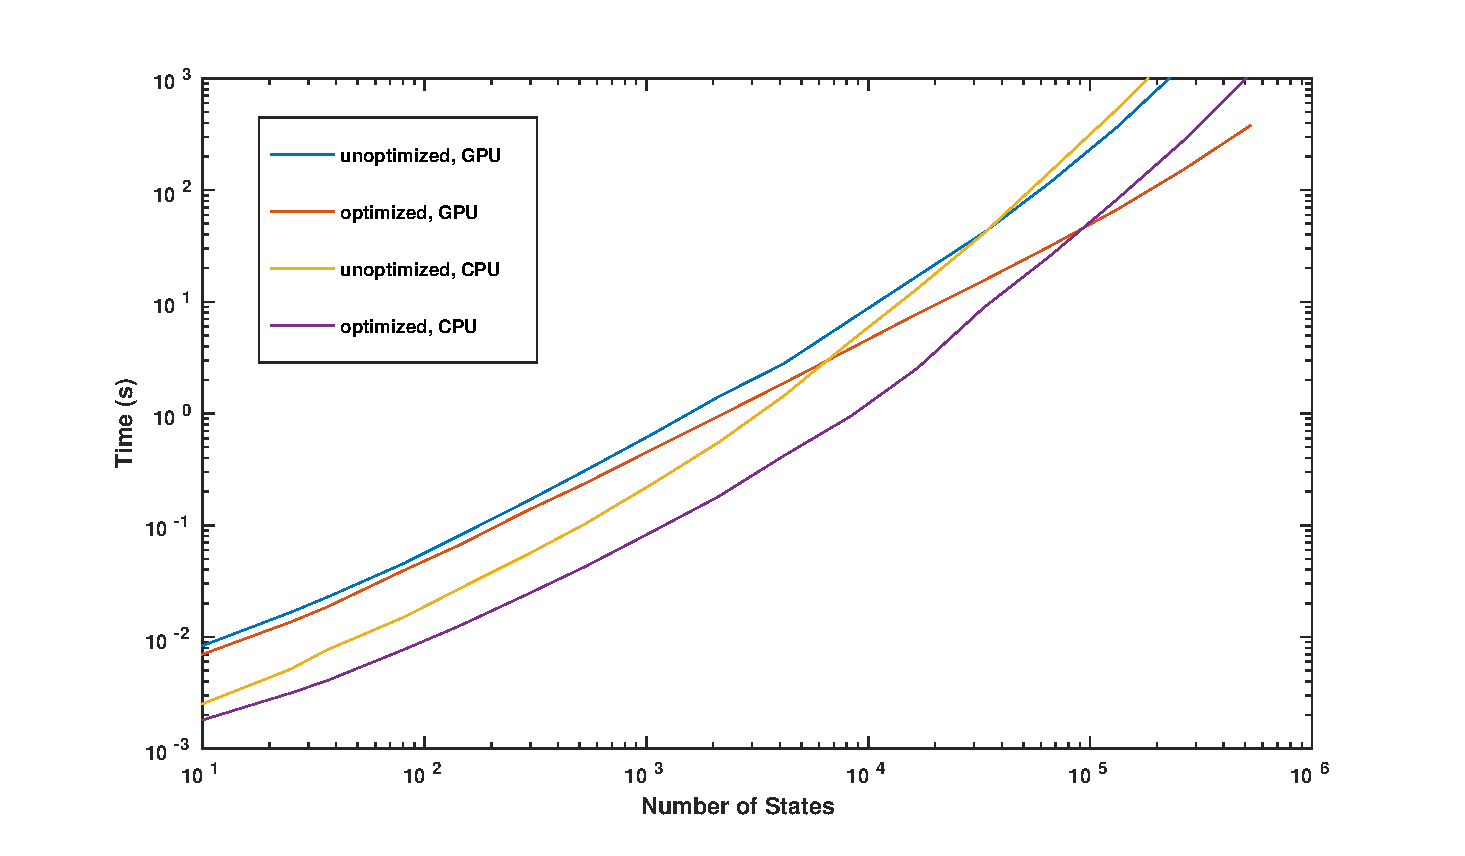
\includegraphics[width=5in]{figures/efficiency2.eps}
\caption{Runtime algorithm X is optimized. } 
\label{fig:desirabilityfunction}
\end{figure}

\begin{table}[]
\centering
\caption{My caption}
\label{my-label}
\begin{tabular}{@{}lllll@{}}
States & A + GPU & B + GPU & A + CPU & B + CPU \\ \midrule
9        & 0.005	& 0.005	& 0.002 & 0.001 \\
25       & 0.007	& 0.006	& 0.002 & 0.001 \\
36       & 0.016	& 0.013	& 0.005 & 0.003 \\
81       & 0.022	& 0.018	& 0.007 & 0.004 \\
144      & 0.045	& 0.039	& 0.015 & 0.007 \\
289      & 0.081	& 0.066	& 0.027 & 0.012 \\
529      & 0.163	& 0.134	& 0.054	& 0.023 \\
1089     & 0.308	& 0.236	& 0.102	& 0.042 \\
2116     & 0.670	& 0.489	& 0.241	& 0.089 \\
4160     & 1.414	& 0.946	& 0.551	& 0.180 \\
8372     & 2.794	& 1.871	& 1.436	& 0.418 \\
16640    & 6.952	& 3.841	& 4.465	& 0.951 \\
33304    & 16.99	& 7.819	& 13.10	& 2.541 \\
65786    & 41.83	& 15.56	& 41.22	& 8.929 \\
132120   & 116.5	& 31.38	& 145.3	& 25.63 \\
262626   & 365.9	& 66.91	& 528.5	& 82.57 \\
526294   & 1304	& 151.5	& 2053.	& 275.2 \\
1050504  & 5492	& 376.8	& 7747	& 1084
\end{tabular}
\end{table}
% ====================
\section{Testing Placements on Real World Scenarios}
% ====================

% ====================
\subsection{Data Set}
\label{sec:rgbddataset}
% ====================
A data set of RGBD video is obtained by attaching an Asus Xtion Pro Live onto a
(Wheelchair Model) power wheelchair. Obstacles such as chairs, other
wheelchairs, tables and cabinets are laid out in an indoor office environment to
simulate instances where a wheelchair would potentially park.

[x] different instances are recorded. In each instance, the wheelchair starts
from afar, and is drive into the parking spot, reversed out, then moved
laterally and rotationally. At every point in the video, the position of the
parking spot is within sight of the camera, with the assumption that the back-in
algorithm will only be run if the wheelchair is already pointed in the general
area.

A 3D model of the wheelchair used is also obtained using the Kinect Fusion
algorithm [cite]. This allows for precise measurements of how large the
wheelchair is.

\begin{figure}
\centering
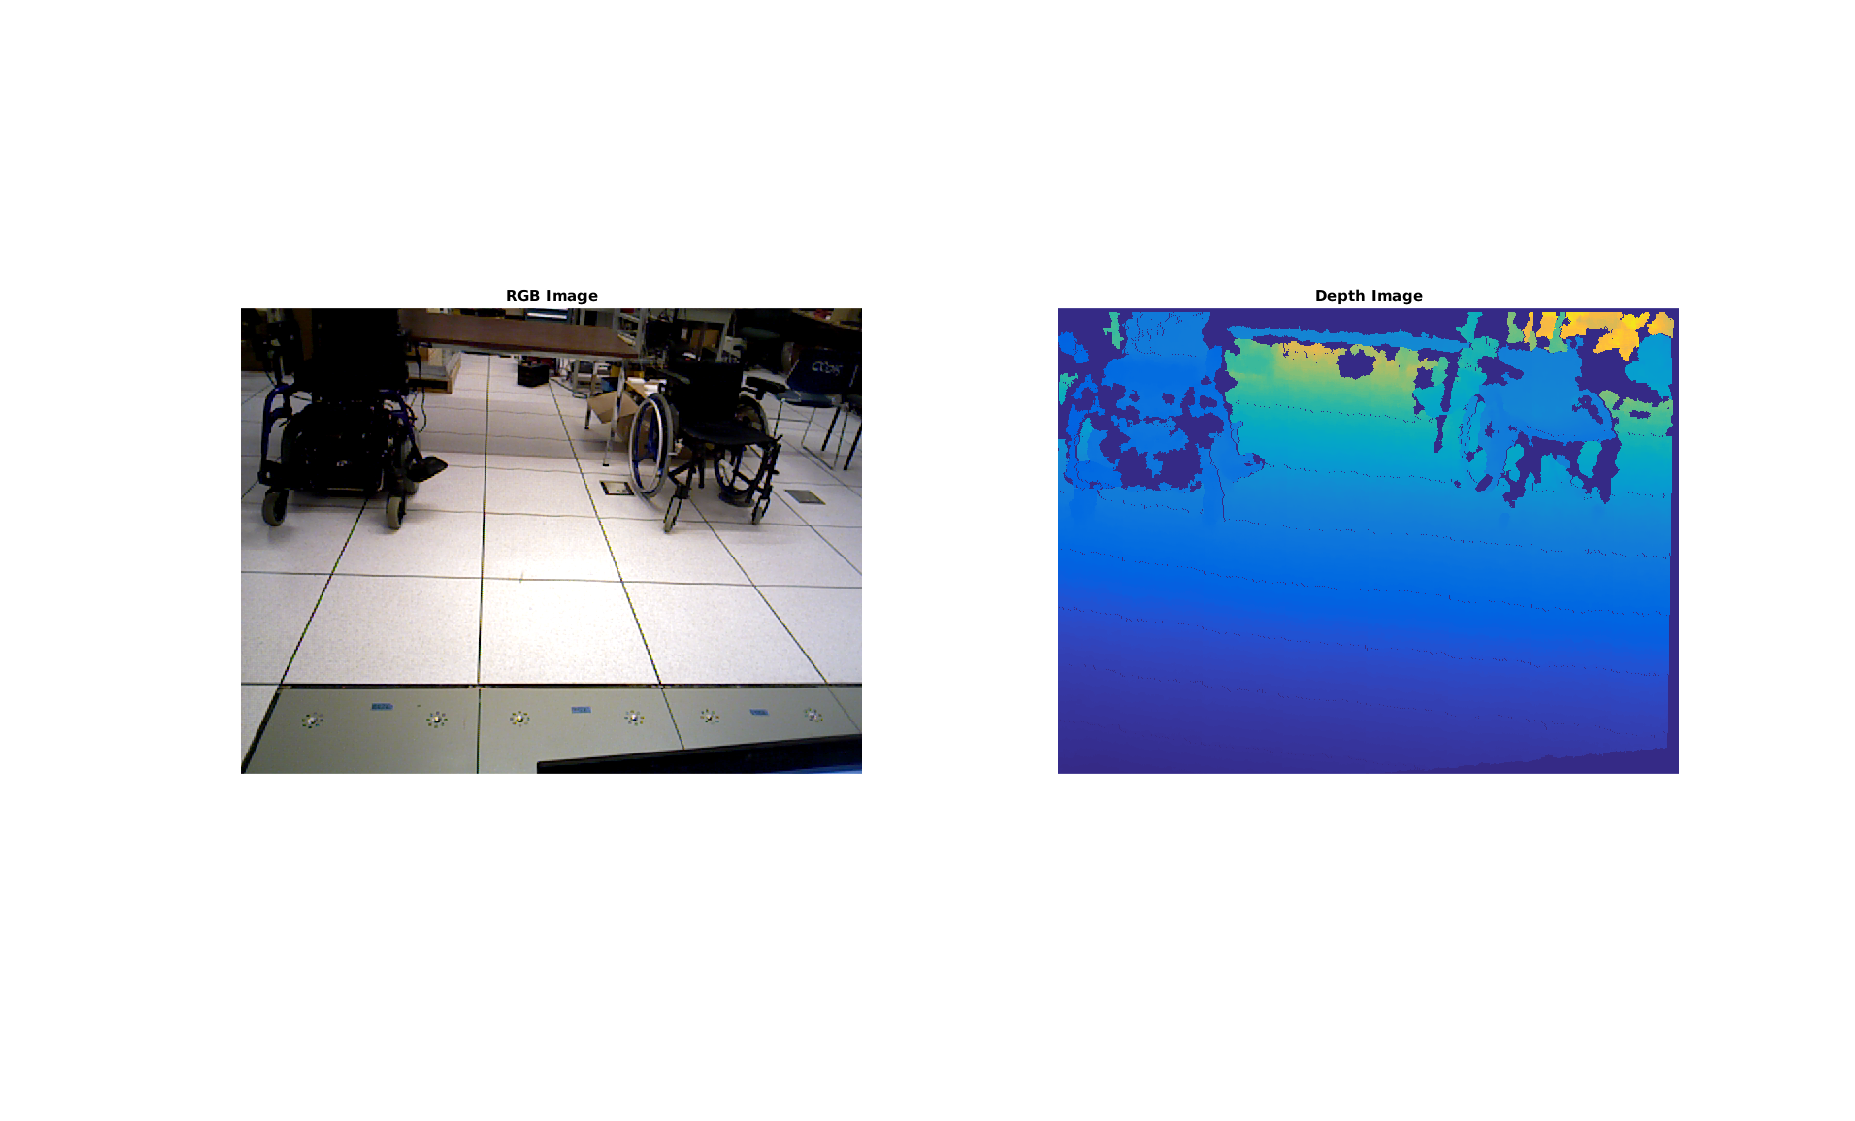
\includegraphics[width=3in]{figures/rgbdwheelchair.png}
\caption{RGB and Depth images as seen by the wheelchair. The objective is to
identify a suitable location within the image for back-in parking.}
\label{fig:rgbdwheelchair}
\end{figure}

% ====================
\subsection{Qualitative Results}
% ====================
5 scenes. For each: RGBD, Placement in Map, Placement in 3D point cloud.

% ====================
\section{Testing Packing Performance}
% ====================
\subsection{Real-World Environments}

\subsection{2D Knapsack Problem}

% ====================
\section{Extension: Placing Wheelchairs so all previous wheelchairs can exit}
% ====================


% ====================
\section{Conclusion}
% ====================

We show our algorithm qualitiatively places objects in spots that minimizes
obstructions.

We formulate an algorithm for efficient computation of the value function, which
is runs in less than 10 seconds.

Performs well as a greedy packing problem heuristic.

% ======================
\endinput
Any text after an \endinput is ignored.
% ======================
\subsection{Definitions}
TODO put closer to where it's used

\begin{itemize}
\item Configuration space
\item Pointcloud space
\item 2D Map space
\item Ground Map
\item Object Map
\item Unknown Map
\item Feasible states
\item Desirability function
\end{itemize}
